\documentclass[first=dgreen,second=purple,logo=redexc]{aaltoslides}
%\documentclass{aaltoslides} % DEFAULT
%\documentclass[first=purple,second=lgreen,logo=redque,normaltitle,nofoot]{aaltoslides} % SOME OPTION EXAMPLES

\usepackage[latin9]{inputenc}
\usepackage[T1]{fontenc}
\usepackage{graphicx}
\usepackage{amssymb,amsmath}
\usepackage{url}
\usepackage{lastpage}
\usepackage{array}
\usepackage{amsbsy}
\usepackage{multirow}
\usepackage[absolute,overlay]{textpos}
\usepackage{soul}

\newcolumntype{x}[1]{%
>{\centering\hspace{0pt}}p{#1}}%

\makeatletter
\def\thickhrulefill{\leavevmode \leaders \hrule height 1ex \hfill \kern \z@}
\def\@makechapterhead#1{%
  %\vspace*{50\p@}%
  \vspace*{11\p@}%
  {\parindent \z@ \centering \reset@font
        \thickhrulefill\quad
        \scshape \@chapapp{} \thechapter
        \quad \thickhrulefill
        \par\nobreak
        \vspace*{11\p@}%
        \interlinepenalty\@M
        \hrule
        \vspace*{11\p@}%
        \Huge \bfseries #1\par\nobreak
        \par
        \vspace*{11\p@}%
        \hrule
    %\vskip 40\p@
    \vskip 90\p@
  }}

%from here 
% fquote Fancy Quotation environment

% Use \sloppy to make right-margin easier?
% Set picture units to be relative to font size (em)?
% Use begingroup to rest units afterwards?

\newcommand{\fq@author}{}
\newcommand*{\fqsource}[1]{\gdef\fq@source{#1}}
\definecolor{quotemark}{gray}{0.7}

\newenvironment{fquote}[1][]{%
\def\fq@author{#1}% Seem to need to use def for ifx @empty to work
\let\fq@source\@empty
  \vspace{1em}
  \begin{list}{}{%
      \setlength{\leftmargin}{0.2\textwidth}
      \setlength{\rightmargin}{0.2\textwidth}
    }
    \item[]%
    \begin{picture}(0,0)(0,0)
      \put(-15,-5){\makebox(0,0){%
	  \scalebox{5}{\textcolor{quotemark}{\bfseries``}}}%
      }
    \end{picture}\em\ignorespaces%
}{%
  \newline%
  \makebox[0pt][l]{\hspace{0.6\textwidth}%
  \begin{picture}(0,0)(0,0)
    \put(15,10){\makebox(0,0){%
	\scalebox{5}{\textcolor{quotemark}{\rm\bfseries''}}}%
    }
  \end{picture}}%
  \ifx\fq@author\@empty\else\hfill\textsc{--- \fq@author}\fi
  \ifx\fq@source\@empty\else\\\mbox{}\hfill\textsl{\small\fq@source}\fi
  \end{list}
  \ifx\fq@author\@empty\else\vspace{1em}\fi
}
%to here

% Synopsis environment (like an abstract for each chapter)

\newcommand{\synopsisname}{Synopsis}

\newenvironment{synopsis}{%
%  \small
  \begin{center}%
    {\bfseries \synopsisname\vspace{-.5em}\vspace{\z@}}%
  \end{center}%
  \quotation
}{%
  \endquotation
}

\newenvironment{publish}{%
  \vfil
  \center\small\ignorespaces
  \rule{10em}{0.4pt}\par\noindent\ignorespaces
}{%
  \par\noindent\rule[1ex]{10em}{0.4pt}
  \endcenter
}


\makeatletter
% \renewcommand\bibsection%
% {
%   \section*{\refname
%     \@mkboth{\MakeUppercase{\refname}}{\MakeUppercase{\refname}}}
% }

\makeatother
% \fancyhf{} % delete current setting for header and footer
% \fancyhead{} % get rid of headers on plain pages
% %\renewcommand{\chaptermark}[1]{\markboth{#1}{}}
% \renewcommand{\sectionmark}[1]{\markright{#1}{}}
% \fancyhead[RE]{\sffamily\nouppercase{\rightmark} }
% \fancyhead[LO]{\sffamily\nouppercase{\leftmark} }
% %\fancyfoot[RO, LE] {\thepage}
% \fancyfoot[C]{\thepage}
%\headrulewidth 0.4pt
%\footrulewidth 0 pt


\title{Mixture Models from Multiresolution data}

\author[Prem Raj Adhikari]{ Prem Raj Adhikari$^{1,2}$}
\institute[ICS]{ \hspace{0.5mm} Parsimonious Modeling Research Group in \\
$^{1}$Department of Information and Computer Science\\
\hspace{1.5mm}Aalto University School of Science, Finland\\
$^{2}$Helsinki Institute for Information Technology (HIIT) \\
%\hspace{1.5mm}Helsinki, Finland  \\
\hspace{1.5mm}prem.adhikari@aalto.fi }

\aaltofootertext{Mixture Models from Multiresolution 0--1 data} 
{Summer Seminar, August 20, 2013}
{Kuopio, \insertframenumber/\inserttotalframenumber}

%\date{November 2--4, 2011}
\makeatletter

\newcommand\FrameText[1]{%
  \begin{textblock*}{0.98\textwidth}(0.2\textwidth,0.95\textheight)
    \textcolor {blue}{\scriptsize\raggedright #1\hspace{0.1\textwidth}}
  \end{textblock*}}

\begin{document}
%%%%%%%%%%%%%%%%%%%%%%%%%%%%%%%%%%%%%%%%%%%%%%%%%%%%%%%%%%%%%%%%%%%%%%%%%%%%%%%%%%%%%%%%%%%%%

\aaltotitleframe

%%%%%%%%%%%%%%%%%%%%%%%%%%%%%%%%%%%%%%%%%%%%%%%%%%%%%%%%%%%%%%%%%%%%%%%%%%%%%%%%%%%%%%%%%%%%%

% \begin{frame}
%   \frametitle{Outline}
%   \tableofcontents%[pausesections]
% 
% \end{frame}

% %%%%%%%%%%%%%%%%%%%%%%%%%%%%%%%%%%%%%%%%%%%%%%%%%%%%%%%%%%%%%%%%%%%%%%%%%%%%%%%%%%%%%%%%%%%%%
\begin{frame}{Management Summary}
\begin{itemize} \setlength{\itemsep}{6.5mm}
  \item Motivation for the Work 
  \item Multiresolution Data
  \item Algorithms and Experiments 
  \item Summary and Conclusions
\end{itemize}
\end{frame}



% %%%%%%%%%%%%%%%%%%%%%%%%%%%%%%%%%%%%%%%%%%%%%%%%%%%%%%%%%%%%%%%%%%%%%%%%%%%%%%%%%%%%%%%%%%%%%
% 
% 
% \begin{frame} {Motivations: The hi/story of Tobias Mayer} 
% 
% \begin{figure}
% \centering
%   \includegraphics[width=0.5\textwidth]{figures/mayer}
% \end{figure}
% 
% \hspace{40mm} Tobias Mayer 
% \end{frame}
% 
% %%%%%%%%%%%%%%%%%%%%%%%%%%%%%%%%%%%%%%%%%%%%%%%%%%%%%%%%%%%%%%%%%%%%%%%%%%%%%%%%%%%%%%%%%%%%%
% 
% \begin{frame} {Motivations: Motions of the moon} 
% 
% \begin{figure}
% \centering
%   \includegraphics[width=0.5\textwidth]{figures/fullmoon}
% \end{figure}
% 
% \hspace{30mm} Moon wobbles every month 
% \end{frame}
% 
% %%%%%%%%%%%%%%%%%%%%%%%%%%%%%%%%%%%%%%%%%%%%%%%%%%%%%%%%%%%%%%%%%%%%%%%%%%%%%%%%%%%%%%%%%%%%%
% 
% 
% \begin{frame} {Motivations: Motions of the moon} 
% 
% \begin{figure}
% \centering
%   \includegraphics[trim=1cm 1cm 1cm 1cm, clip=true, width=0.7\textwidth]{figures/earthrotation}
% \end{figure}
% \hspace{18mm}  Orbit of the Moon is not a perfect circle
% \end{frame}
% 
% %%%%%%%%%%%%%%%%%%%%%%%%%%%%%%%%%%%%%%%%%%%%%%%%%%%%%%%%%%%%%%%%%%%%%%%%%%%%%%%%%%%%%%%%%%%%%
% 
% \begin{frame} {Motivations: Motions of the moon} 
% 
% \begin{figure}
% \centering
%   \includegraphics[width=\textwidth]{figures/earthrotationex}
% \end{figure}
% \hspace{15mm}  Orbit of the Moon is not a perfect circle
% \end{frame}
% 
% %%%%%%%%%%%%%%%%%%%%%%%%%%%%%%%%%%%%%%%%%%%%%%%%%%%%%%%%%%%%%%%%%%%%%%%%%%%%%%%%%%%%%%%%%%%%%
% 
% \begin{frame} {Motivations: Motions of the moon} 
% 
% \begin{figure}
% \centering
%   \includegraphics[width=0.9\textwidth]{figures/sunnn2}
% \end{figure}
% \scriptsize  \hspace{18mm}  Axis of the moon's rotation is not exactly perpendicular
% \end{frame}
% 
% %%%%%%%%%%%%%%%%%%%%%%%%%%%%%%%%%%%%%%%%%%%%%%%%%%%%%%%%%%%%%%%%%%%%%%%%%%%%%%%%%%%%%%%%%%%%%
% 
% \begin{frame} {Motivations: Motions of the moon} 
% 
% \begin{figure}
% \centering
%   \includegraphics[width=0.5\textwidth]{figures/fullmoon}
% \end{figure}
% \scriptsize \hspace{27mm} Mayer looked at the surface of the moon
% \end{frame}
% 
% %%%%%%%%%%%%%%%%%%%%%%%%%%%%%%%%%%%%%%%%%%%%%%%%%%%%%%%%%%%%%%%%%%%%%%%%%%%%%%%%%%%%%%%%%%%%%
% 
% \begin{frame} {Motivations: Motions of the moon} 
% 
% \begin{figure}
% \centering
%   \includegraphics[width=0.65\textwidth]{figures/fullmoonnnn}
% \end{figure}
% %\hspace{15mm} Bright 
% \end{frame}
% 
% %%%%%%%%%%%%%%%%%%%%%%%%%%%%%%%%%%%%%%%%%%%%%%%%%%%%%%%%%%%%%%%%%%%%%%%%%%%%%%%%%%%%%%%%%%%%%
% 
% \begin{frame} {Motivations: Math behind Libration of the moon} 
% 
% {\Huge 
% $ \beta - x = y \alpha - z \alpha \sin \theta$}
% \end{frame}
% 
% %%%%%%%%%%%%%%%%%%%%%%%%%%%%%%%%%%%%%%%%%%%%%%%%%%%%%%%%%%%%%%%%%%%%%%%%%%%%%%%%%%%%%%%%%%%%%
% 
% \begin{frame} {Motivations: Math behind Libration of the moon} 
% 
% {\Huge 
% $ \beta - {\color {red}x} = {\color {red}y} \alpha - {\color {red}z} \alpha \sin \theta$
% 
% \hspace{13.5mm} $\Uparrow $ \hspace{5.7mm} $\Uparrow$ \hspace{11.4mm}  $\Uparrow $}
% \end{frame}
% 
% %%%%%%%%%%%%%%%%%%%%%%%%%%%%%%%%%%%%%%%%%%%%%%%%%%%%%%%%%%%%%%%%%%%%%%%%%%%%%%%%%%%%%%%%%%%%%
% 
% \begin{frame} {Motivations: Math behind Libration of the moon} 
% 
% {\Huge
% $\Downarrow $ \hspace{27.5mm} $\Downarrow$ \hspace{11.2mm}  $\Downarrow $ \hspace{8.4mm}  $\Downarrow $
% 
% $ {\color {red}\beta} - x = y {\color {red}\alpha} - z {\color {red}\alpha} \sin {\color {red}\theta}$ }
% 
% %\hspace{5mm} $\Uparrow $ \hspace{15mm} $\Uparrow$ \hspace{20mm}  $\Uparrow $
% \end{frame}
% %%%%%%%%%%%%%%%%%%%%%%%%%%%%%%%%%%%%%%%%%%%%%%%%%%%%%%%%%%%%%%%%%%%%%%%%%%%%%%%%%%%%%%%%%%%%%
% 
% \begin{frame} {Motivations: Math behind Libration of the moon} 
% 
% {\Large
% $\beta - 13 ^\circ 10' = 0.8836 \alpha - 0.4682 \alpha \sin \theta $ 
% 
% \vspace{4mm}
% 
% $\beta - 13 ^\circ 08' = 0.9996 \alpha - 0.0282 \alpha \sin \theta $ 
% 
% \vspace{4mm}
% 
% $\beta - 13 ^\circ 12' = 0.9899 \alpha - 0.1421 \alpha \sin \theta $ }
% 
% \end{frame}
% %%%%%%%%%%%%%%%%%%%%%%%%%%%%%%%%%%%%%%%%%%%%%%%%%%%%%%%%%%%%%%%%%%%%%%%%%%%%%%%%%%%%%%%%%%%%%
% 
% \begin{frame} {Motivations: Math behind Libration of the moon} 
% 
% \scriptsize 
% $\beta - 13 ^\circ 10' = 0.8836 \alpha - 0.4682 \alpha \sin \theta $ \hspace{5mm} $\beta - 13 ^\circ 02' = 0.9996 \alpha - 0.0282 \alpha \sin \theta $ 
% 
% $\beta - 13 ^\circ 08' = 0.9996 \alpha - 0.0282 \alpha \sin \theta $ \hspace{5mm} $\beta - 13 ^\circ 02' = 0.9996 \alpha - 0.0282 \alpha \sin \theta $ 
% 
% $\beta - 13 ^\circ 12' = 0.9899 \alpha - 0.1421 \alpha \sin \theta $ \hspace{5mm} $\beta - 13 ^\circ 02' = 0.9996 \alpha - 0.0282 \alpha \sin \theta $ 
% 
% $\beta - 13 ^\circ 01' = 0.9899 \alpha - 0.1421 \alpha \sin \theta $ \hspace{5mm} $\beta - 13 ^\circ 02' = 0.9996 \alpha - 0.0282 \alpha \sin \theta $ 
% 
% $\beta - 13 ^\circ 05' = 0.8836 \alpha - 0.4682 \alpha \sin \theta $ \hspace{5mm} $\beta - 13 ^\circ 02' = 0.9996 \alpha - 0.0282 \alpha \sin \theta $ 
% 
% $\beta - 13 ^\circ 02' = 0.9996 \alpha - 0.0282 \alpha \sin \theta $ \hspace{5mm} $\beta - 13 ^\circ 02' = 0.9996 \alpha - 0.0282 \alpha \sin \theta $ 
% 
% $\beta - 13 ^\circ 12' = 0.9899 \alpha - 0.1421 \alpha \sin \theta $ \hspace{5mm} $\beta - 13 ^\circ 02' = 0.9996 \alpha - 0.0282 \alpha \sin \theta $ 
% 
% $\beta - 13 ^\circ 11' = 0.9899 \alpha - 0.1421 \alpha \sin \theta $ \hspace{5mm} $\beta - 13 ^\circ 02' = 0.9996 \alpha - 0.0282 \alpha \sin \theta $ 
% 
% $\beta - 13 ^\circ 07' = 0.8836 \alpha - 0.4682 \alpha \sin \theta $ \hspace{5mm} $\beta - 13 ^\circ 02' = 0.9996 \alpha - 0.0282 \alpha \sin \theta $ 
% 
% $\beta - 13 ^\circ 15' = 0.9996 \alpha - 0.0282 \alpha \sin \theta $ \hspace{5mm} $\beta - 13 ^\circ 02' = 0.9996 \alpha - 0.0282 \alpha \sin \theta $ 
% 
% $\beta - 13 ^\circ 42' = 0.9899 \alpha - 0.1421 \alpha \sin \theta $ \hspace{5mm} $\beta - 13 ^\circ 02' = 0.9996 \alpha - 0.0282 \alpha \sin \theta $ 
% 
% $\beta - 13 ^\circ 31' = 0.9899 \alpha - 0.1421 \alpha \sin \theta $ \hspace{5mm} $\beta - 13 ^\circ 02' = 0.9996 \alpha - 0.0282 \alpha \sin \theta $ 
% 
% $\beta - 13 ^\circ 34' = 0.8836 \alpha - 0.4682 \alpha \sin \theta $ \hspace{5mm} $\beta - 13 ^\circ 02' = 0.9996 \alpha - 0.0282 \alpha \sin \theta $ 
% 
% $\beta - 13 ^\circ 53' = 0.9996 \alpha - 0.0282 \alpha \sin \theta $ 
% 
% 
% \end{frame}
% %%%%%%%%%%%%%%%%%%%%%%%%%%%%%%%%%%%%%%%%%%%%%%%%%%%%%%%%%%%%%%%%%%%%%%%%%%%%%%%%%%%%%%%%%%%%%
% 
% \begin{frame} {Motivations: Math behind Libration of the moon} 
% 
% \begin{figure}
% \centering
%   \includegraphics[trim=1cm 1cm 1cm 1cm, clip=true, width=1.05\textwidth]{figures/mooneq}
% \end{figure}
% 
% \end{frame}
% 
% %%%%%%%%%%%%%%%%%%%%%%%%%%%%%%%%%%%%%%%%%%%%%%%%%%%%%%%%%%%%%%%%%%%%%%%%%%%%%%%%%%%%%%%%%%%%%%%%%%%%%%%%%%%%%%%%%%%%%%%%%%%%%%%%%%%%%%%%%%%%%%%%%
% 
% 
% 
% \begin{frame} {Motivations: Math behind Libration of the moon} 
% 
% \tiny
% \hspace{1mm}$\beta - 13 ^\circ 10' = +0.8836 \alpha - 0.4682 \alpha \sin \theta $ \hspace{12mm} $\beta - 13 ^\circ 02' = -0.1570 \alpha - 0.9876 \alpha \sin \theta $ 
% 
% \hspace{1mm}$\beta - 13 ^\circ 08' = +0.9996 \alpha - 0.0282 \alpha \sin \theta $ \hspace{12mm} $\beta - 13 ^\circ 02' = -0.3363 \alpha - 0.9418 \alpha \sin \theta $ 
% 
% \hspace{1mm}$\beta - 13 ^\circ 12' = +0.9899 \alpha - 0.1421 \alpha \sin \theta $ \hspace{12mm} $\beta - 13 ^\circ 02' = -0.8560 \alpha - 0.5170 \alpha \sin \theta $ 
% 
% \hspace{1mm}$\beta - 13 ^\circ 01' = +0.9308 \alpha - 0.3654 \alpha \sin \theta $ \hspace{12mm} $\beta - 13 ^\circ 02' = -0.9952 \alpha - 0.0982 \alpha \sin \theta $ 
% 
% \hspace{1mm}$\beta - 13 ^\circ 05' = +0.9097 \alpha - 0.4152 \alpha \sin \theta $ \hspace{12mm} $\beta - 13 ^\circ 02' = -0.8409 \alpha - 0.5412 \alpha \sin \theta $ 
% 
% \hspace{1mm}$\beta - 13 ^\circ 02' = +1.0000 \alpha - 0.0055 \alpha \sin \theta $ \hspace{12mm} $\beta - 13 ^\circ 02' = -0.9429 \alpha - 0.3330 \alpha \sin \theta $ 
% 
% \hspace{1mm}$\beta - 13 ^\circ 12' = +0.9689 \alpha - 0.2476 \alpha \sin \theta $ \hspace{12mm} $\beta - 13 ^\circ 02' = -0.9768 \alpha - 0.2141 \alpha \sin \theta $ 
% 
% \hspace{1mm}$\beta - 13 ^\circ 11' = +0.8878 \alpha - 0.4602 \alpha \sin \theta $ \hspace{12mm} $\beta - 13 ^\circ 02' = -0.6262 \alpha - 0.7797 \alpha \sin \theta $ 
% 
% \hspace{1mm}$\beta - 13 ^\circ 07' = +0.9284 \alpha - 0.3716 \alpha \sin \theta $ \hspace{12mm} $\beta - 13 ^\circ 02' = -0.4091 \alpha - 0.9125 \alpha \sin \theta $ 
% 
% \vspace{-2mm} 
% 
% {\color{red} \line(1,0){123} \hspace{12mm} \line(1,0){122} }
% 
% $\mathbf{9\beta - 118 ^\circ 08' = +8.4987 \alpha - 0.7932 \alpha \sin \theta} $ \hspace{10mm} 
% $\mathbf{9\beta - 140 ^\circ 17' = -6.1404 \alpha + 1.7443 \alpha \sin \theta} $ 
% 
% \vspace{3mm}
% 
% \hspace{26mm} $\beta - 13 ^\circ 15' = +0.2221 \alpha - 0.9750 \alpha \sin \theta $  
% 
% \hspace{26mm} $\beta - 13 ^\circ 02' = +0.0006 \alpha - 1.0000 \alpha \sin \theta $ 
% 
% \hspace{26mm} $\beta - 13 ^\circ 42' = +0.0602 \alpha - 0.9982 \alpha \sin \theta $ 
% 
% \hspace{26mm} $\beta - 13 ^\circ 02' = +0.7549 \alpha - 0.6558 \alpha \sin \theta $ 
% 
% \hspace{26mm} $\beta - 13 ^\circ 31' = +0.5755 \alpha - 0.8178 \alpha \sin \theta $ 
% 
% \hspace{26mm} $\beta - 13 ^\circ 02' = +0.3608 \alpha - 0.9326 \alpha \sin \theta $ 
% 
% \hspace{26mm} $\beta - 13 ^\circ 34' = +0.1302 \alpha - 0.9915 \alpha \sin \theta $ 
% 
% \hspace{26mm} $\beta - 13 ^\circ 02' = -0.1068 \alpha - 0.9943 \alpha \sin \theta $ 
% 
% \hspace{26mm} $\beta - 13 ^\circ 53' = +0.8002 \alpha - 0.5997 \alpha \sin \theta $ 
% 
%  \vspace{-6mm}
%  
%  \begin{center}
%  \hspace{-13mm}{\color{red}\line(1,0){120}}
%  \end{center}
%  
%  \vspace{-4mm}
%  
%  \hspace{25mm} $\mathbf{9\beta - 127 ^\circ 08' = +2.7977 \alpha - 7.9649 \alpha \sin \theta} $ 
%  
% \end{frame}
% 
% %%%%%%%%%%%%%%%%%%%%%%%%%%%%%%%%%%%%%%%%%%%%%%%%%%%%%%%%%%%%%%%%%%%%%%%%%%%%%%%%%%%%%%%%%%%%%
% 
% \begin{frame} {Motivations: Math behind Libration of the moon} 
% 
% {\large
% $9\beta - 118 ^\circ 08' = +8.4987 \alpha - 0.7932 \alpha \sin \theta $ 
% 
% \vspace{4mm}
% 
% $9\beta - 140 ^\circ 17' = -6.1404 \alpha + 1.7443 \alpha \sin \theta $ 
% 
% \vspace{4mm}
% 
% $9\beta - 127 ^\circ 08' = +2.7977 \alpha - 7.9649 \alpha \sin \theta $ }
% 
% \begin{fquote}[{T. Mayer}] 
% $\ldots$ because each of these equations has been formed in the most advantageous manner.
% \fqsource{{1750}} \end{fquote} 
% 
% 
% \end{frame}
% %%%%%%%%%%%%%%%%%%%%%%%%%%%%%%%%%%%%%%%%%%%%%%%%%%%%%%%%%%%%%%%%%%%%%%%%%%%%%%%%%%%%%%%%%%%%%
% 
% \begin{frame} {Motivations: Math behind Libration of the moon} 
% 
% 
% \begin{figure}
% \centering
%   \includegraphics[trim=1cm 1cm 1cm 1cm, clip=true, width=1.05\textwidth]{figures/mooneq}
% \end{figure}
% 
% \end{frame}
% 
% %%%%%%%%%%%%%%%%%%%%%%%%%%%%%%%%%%%%%%%%%%%%%%%%%%%%%%%%%%%%%%%%%%%%%%%%%%%%%%%%%%%%%%%%%%%%%%%%%%%%%%%%%%%%%%%%%%%%%%%%%55
% 
% \begin{frame} {Motivations for Multiresolution Modeling} 
% 
% \begin{fquote}[{T. Mayer}] 
% Because these values were derived from nine times as many observations one can therefore conclude that they are nine times more correct.  
% \fqsource{{1750}} \end{fquote} 
% 
% \end{frame}


%%%%%%%%%%%%%%%%%%%%%%%%%%%%%%%%%%%%%%%%%%%%%%%%%%%%%%%%%%%%%%%%%%%%%%%%%%%%%%%%%%%%%%%%%%%%%%%%%%%%%%%%%%%%%%%%%%%%%%%%%%55

\begin{frame}
 \frametitle {Modelling : the general perspectives}
 
 \begin{fquote}[DecisionCraft Inc.]Modeling is like vintage wine; it matures with time. \fqsource{www.decisioncraft.com} \end{fquote}
 
 \pause 
 
 \begin{fquote}[Prem Raj Adhikari] People may mature with time but models mature only with increasing data. \fqsource{PhD Student} \end{fquote}


 
 \end{frame}

%%%%%%%%%%%%%%%%%%%%%%%%%%%%%%%%%%%%%%%%%%%%%%%%%%%%%%%%%%%%%%%%%%%%%%%%%%%%%%%%%%%%%%%%%%%%%%%%%%5555555%%%%%%%%%55


\begin{frame} {Importance of Using More Samples} 

\begin{alertblock}{The Square Root Law}
   $\text{Accuracy of Information} = \sqrt \text{Volume of Information}$
\end{alertblock}


 
 

\end{frame}


%%%%%%%%%%%%%%%%%%%%%%%%%%%%%%%%%%%%%%%%%%%%%%%%%%%%%%%%%%%%%%%%%%%%%
%%%%%%%%%%%%%%%%%%%%%%%%%%%%%%%%%%%%%%%%%%%%%%%%%%%%%%%%%%%%%%%%%%%%%

\begin{frame} {The Multiresolution data} 

\vspace{1mm}

\begin{figure}
\centering
  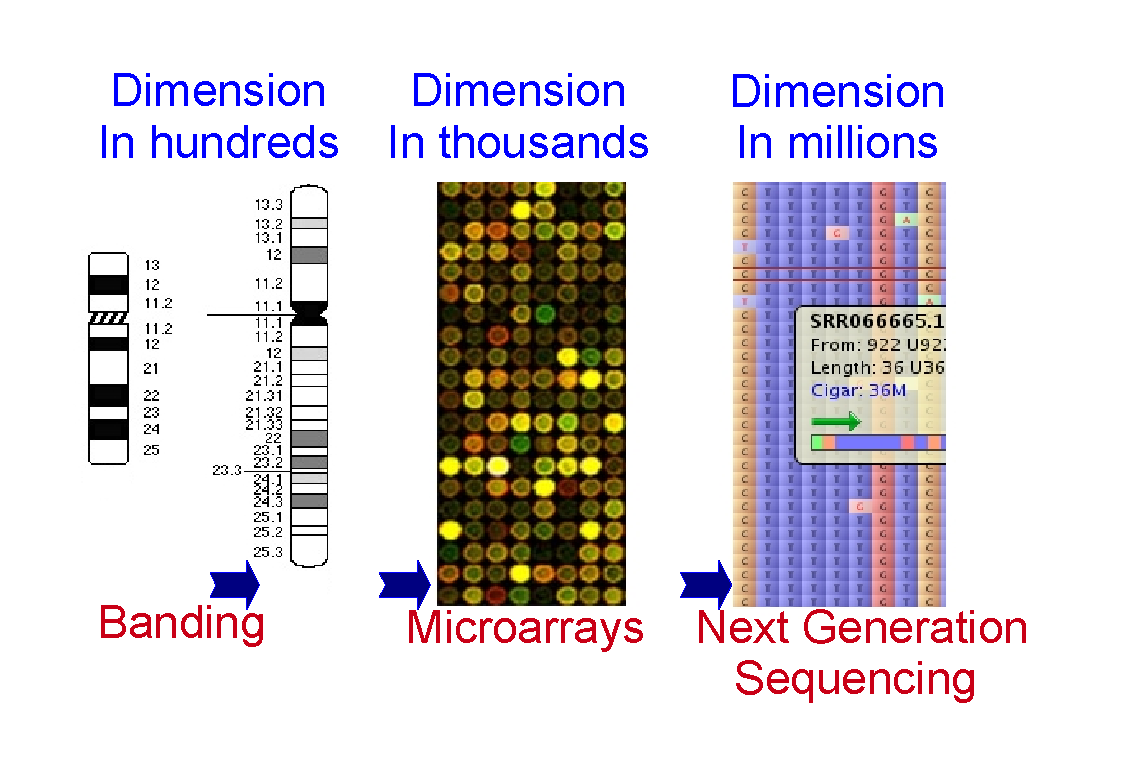
\includegraphics[trim=1cm 1cm 0.5cm 0.5cm, clip=true, width=0.8\textwidth]{figures/multires}
\end{figure}

\vspace{-3mm}

\footnotesize
$\blacksquare$ Multiresolution data is everywhere: biology, computer vision, telecoms ...

$\blacksquare$ Older Generation Technology $\Rightarrow$ Data in Coarse Resolution

$\blacksquare$ Newer Generation Technology $\Rightarrow$ Data in Fine Resolution

\end{frame}
% %%%%%%%%%%%%%%%%%%%%%%%%%%%%%%%%%%%%%%%%%%%%%%%%%%%%%%%%%%%%%%%%%%%%%%%%%%%%%%%%%%%%%%%%%%%%%%%%%%%%%%%%%%%%%%%%%%
% 
% 
% \begin{frame} {Multiresolution Data in Cancer Genomics} 
% 
% 
% \begin{figure}
% \centering
%   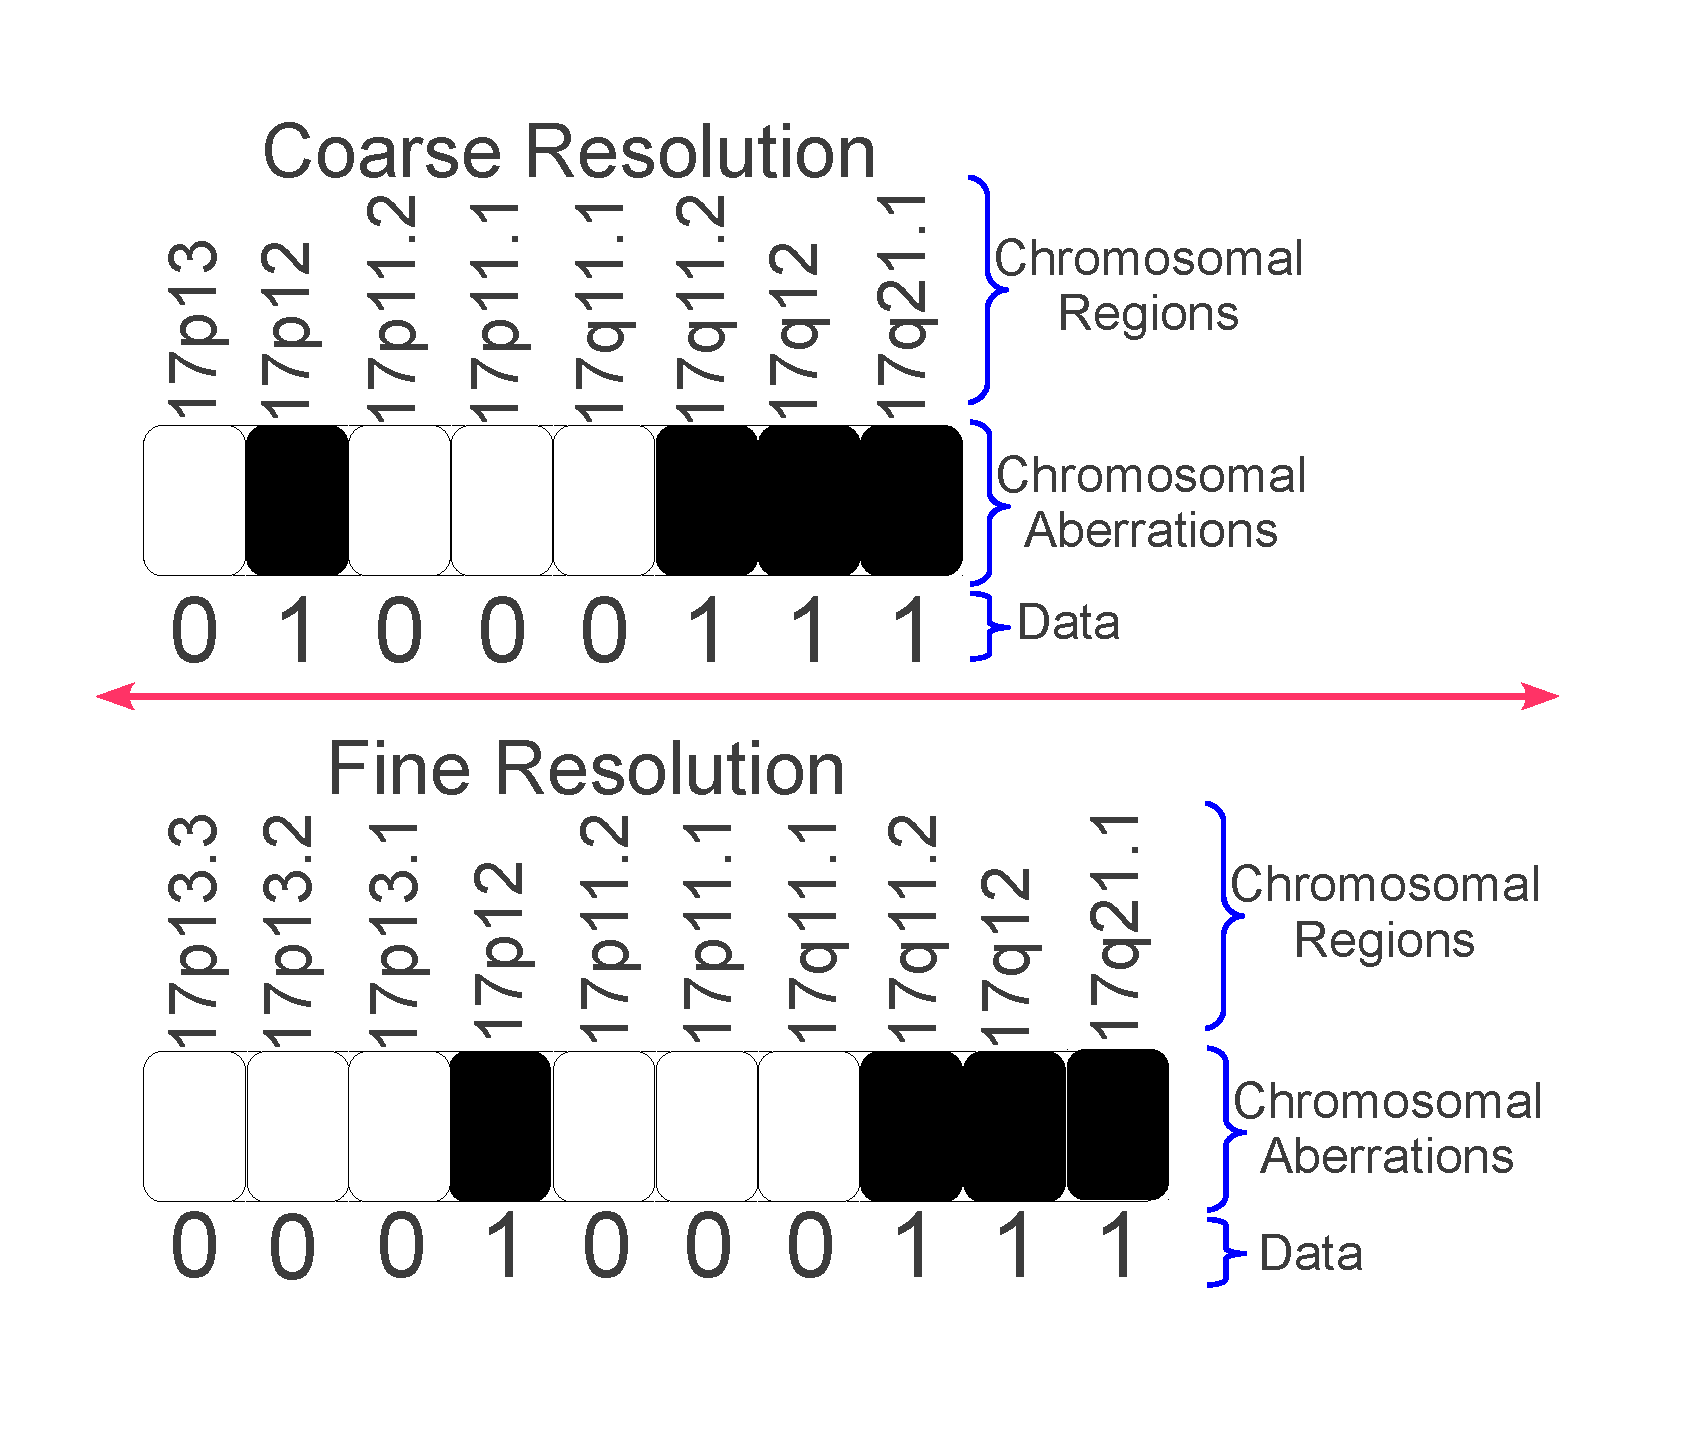
\includegraphics[width=0.8\textwidth]{figures/data}
% \end{figure}
% 
% 
% \end{frame}
%%%%%%%%%%%%%%%%%%%%%%%%%%%%%%%%%%%%%%%%%%%%%%%%%%%%%%%%%%%%%%%%%%%%%%%%%%%%%%%%%%%%%%%%%%%%%%%%%%%%%%%%%%%%%%%%%%%%%%%%

\begin{frame} {Mixture Modeling of Multiresolution 0--1 Data} 
\small
\begin{itemize}\setlength{\itemsep}{1mm}
    \item {\color{red} {Why Mixture Models?}}
    \item Cancer is a heterogeneous collection of several diseases and mixture models are well known for their ability to model heterogeneity
    \item Mixture models generally cannot model multiresolution data
    
    \vspace{-2mm}
    
      \begin{figure}
      \centering
      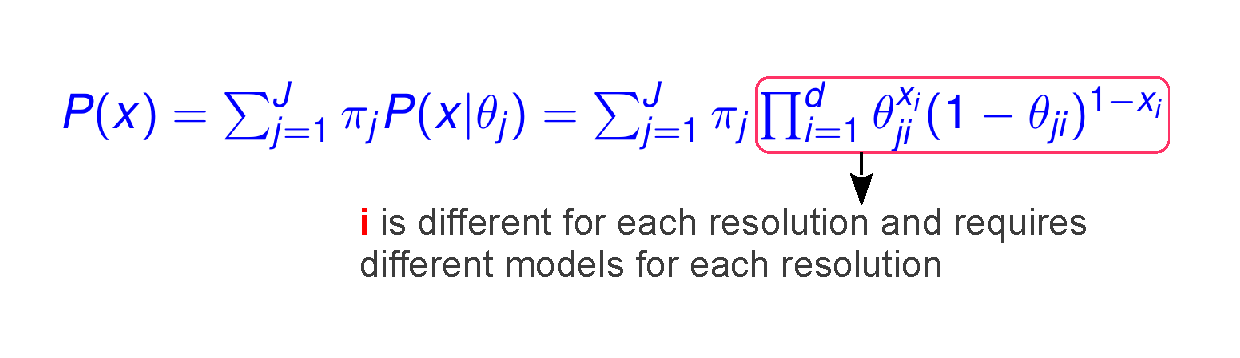
\includegraphics[trim=1cm 1.3cm 1cm 1.3cm, clip=true, width=0.9\textwidth]{figures/multieq}
      \end{figure}
      
          \vspace{-2mm}

     \item Only mixture modeling solution to multiresolution data is to model each resolution separately 
\end{itemize}
\end{frame}

%%%%%%%%%%%%%%%%%%%%%%%%%%%%%%%%%%%%%%%%%%%%%%%%%%%%%%%%%%%%%%%%%%%%%%%%%%%%%%%%%%%%%%%%%%%%%%%%%%%%%%%%%%%%%%%%%%

\begin{frame}{Data transformation for multiresolution modelling}
\begin{figure}
\centering
  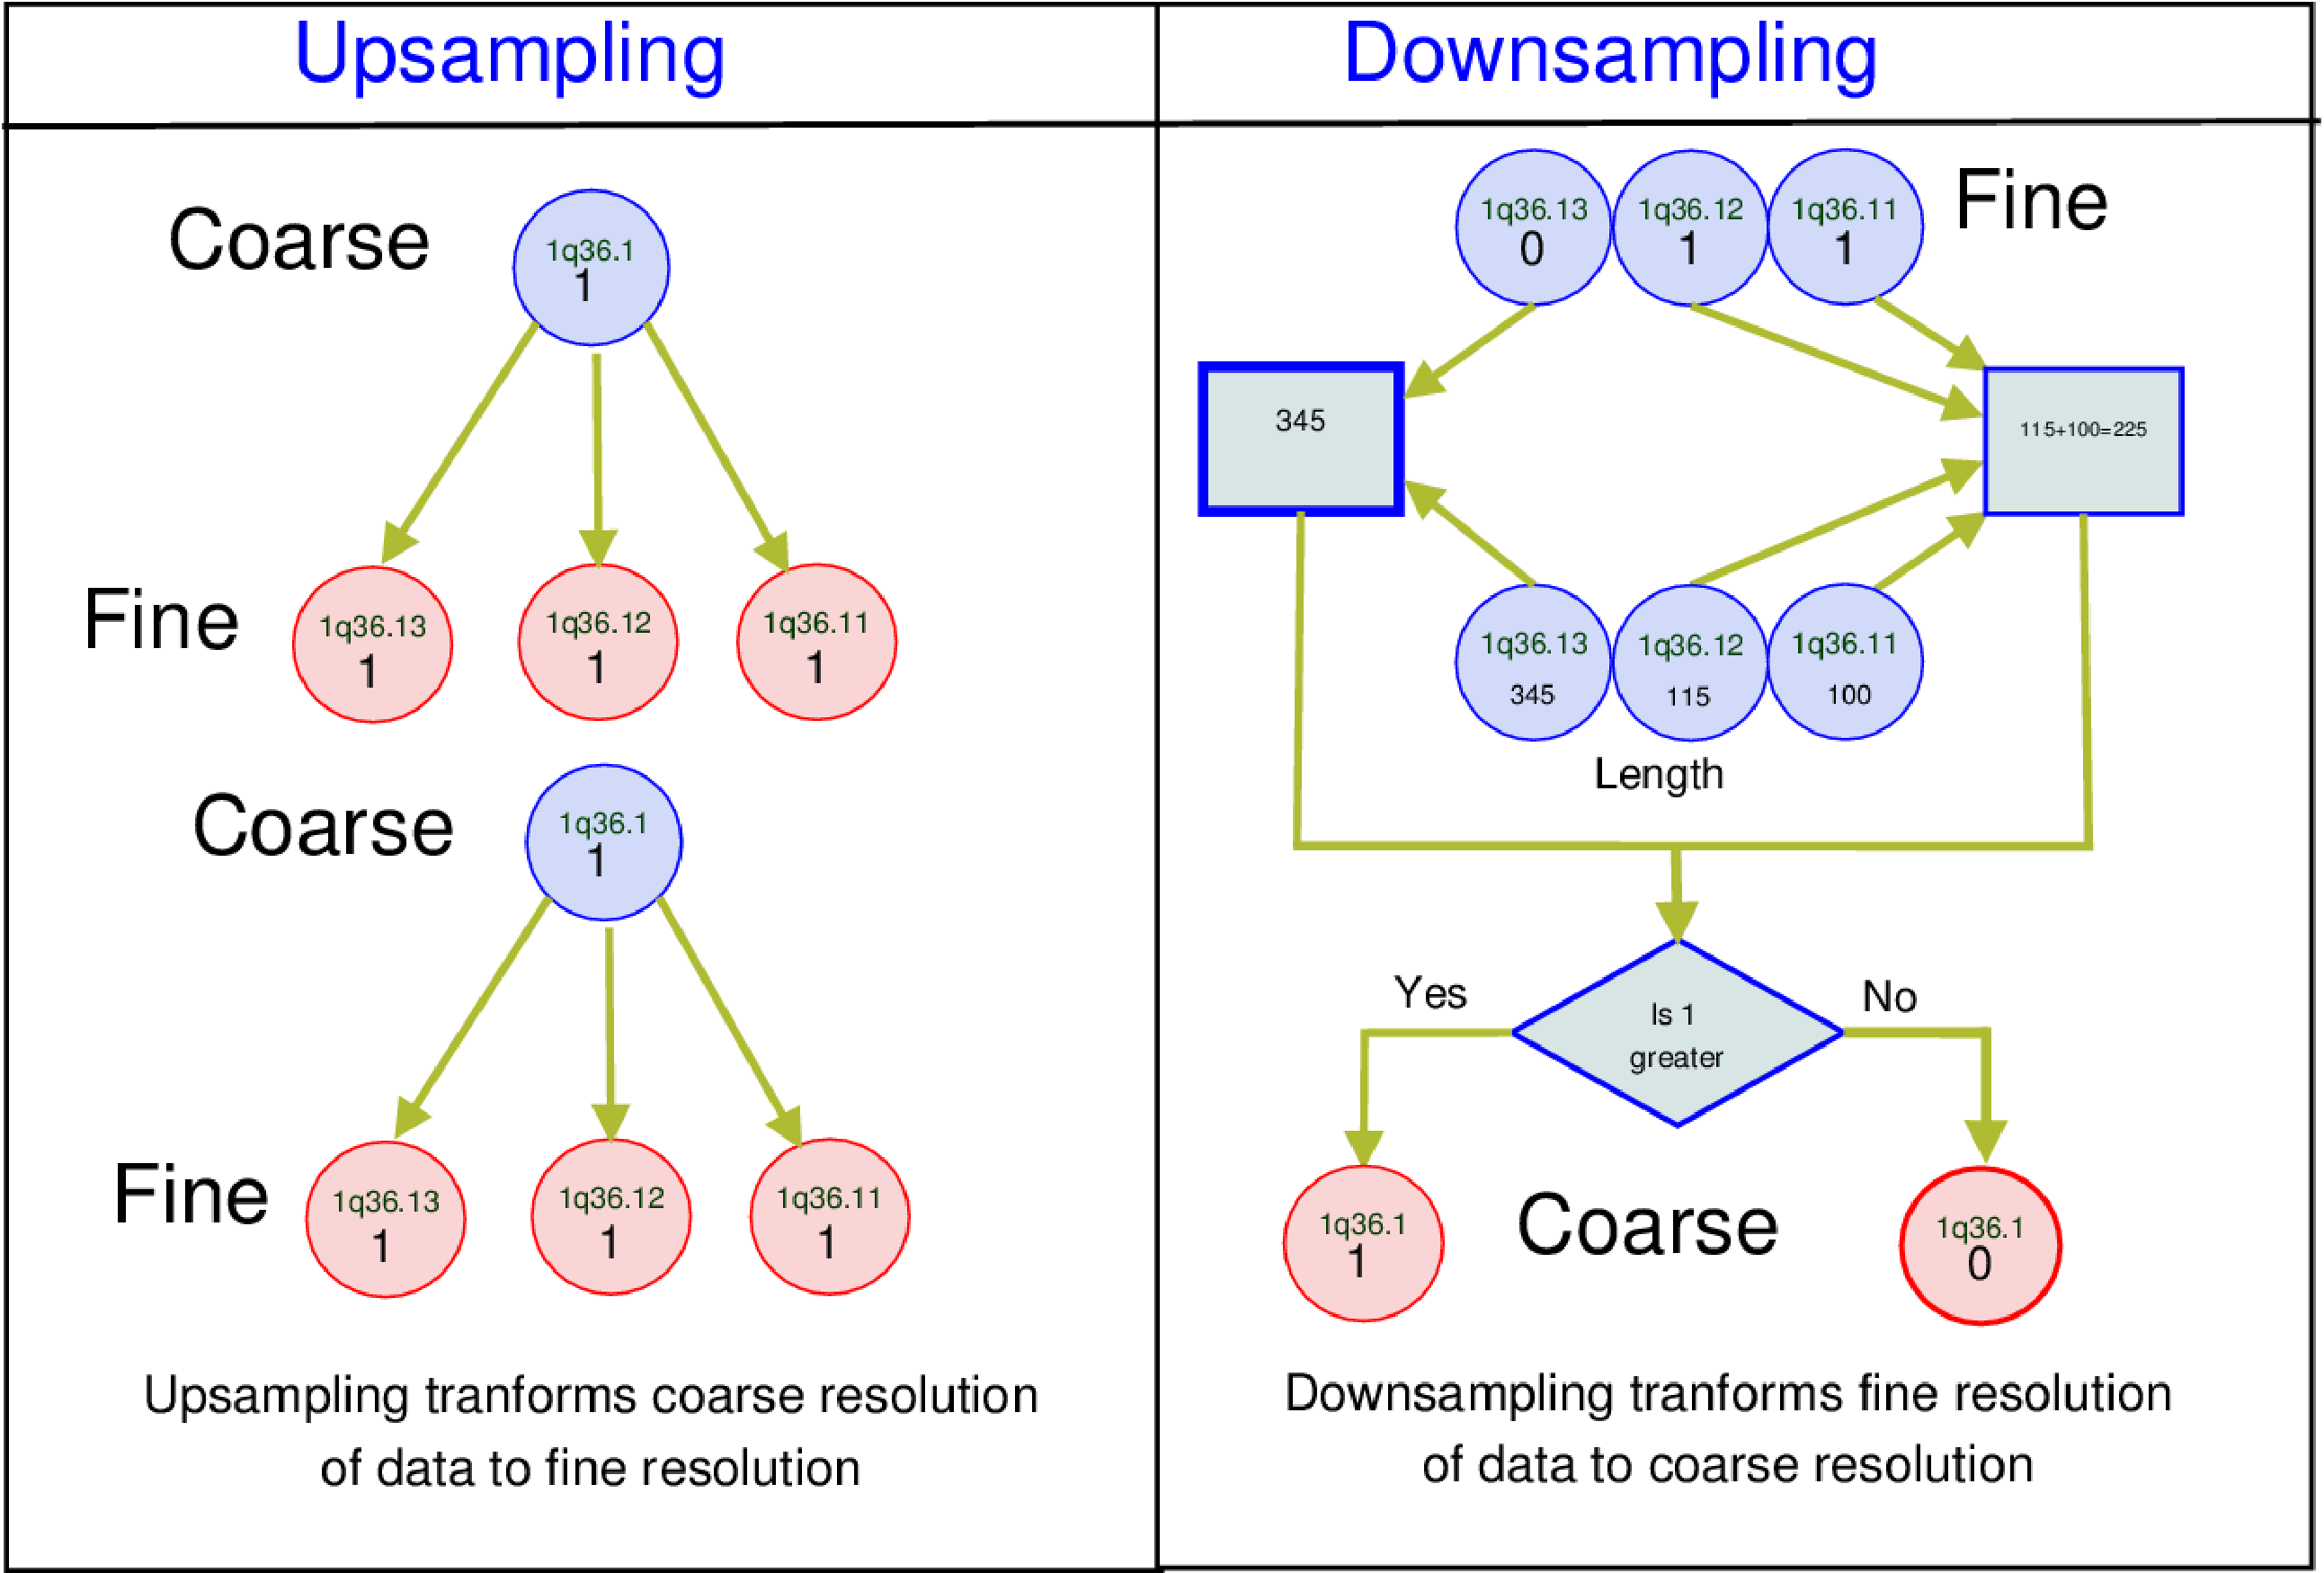
\includegraphics[trim=0cm 0cm 0cm 0cm, clip=true,width=0.60\textwidth]{figures/nweighted}
\end{figure}
\vspace{-5mm}
\scriptsize
We upsample and downsample the data and integrate the data in same resolution before mixture modelling
\FrameText{P. R. Adhikari, J. Hollm{\'e}n, UP'2010 \\ \textbf{Patterns from Multiresolution 0-1 data}}
\end{frame}
%%%%%%%%%%%%%%%%%%%%%%%%%%%%%%%%%%%%%%%%%%%%%%%%%%%%%%%%%%%%%%%%%%%%%%%%%%%%%%%%%%%%%%%%%%%%%

\begin{frame}
\frametitle{Results of Mixture Models}
\begin{table}[h!]
  \centering
  \begin{tabular}{|l|c|c|}
    \hline
    \textbf{Data Resolution} & \textbf{J} &\textbf{Likelihood}  \\
    \hline
    Original in Coarse		&	8	& 	-3.39  \\ \hline
    Original in Fine		&	8	& 	-4.75 \\ \hline
    Downsampled to Coarse	&	6	& 	-3.41  \\ \hline
    Upsampled to Fine		&	6	& 	-5.23  \\ \hline
    Combined  in Coarse 	&	7	& 	-3.36  \\ \hline
    Combined in Fine		&	7	& 	-5.11  \\ \hline     
  \end{tabular}
  \caption{Results of experiments on chromosome-17. J denotes the selected number of component distributions. }\label{Tab:results}
\end{table}
\FrameText{P. R. Adhikari, J. Hollm{\'e}n, UP'2010 \\ \vspace{-2mm} \textbf{Patterns from Multiresolution 0-1 data}}
\end{frame}

%%%%%%%%%%%%%%%%%%%%%%%%%%%%%%%%%%%%%%%%%%%%%%%%%%%%%%%%%%%%%%%%%%%%%%%%%%%%%%%%%%%%%%%%%%%%%

\begin{frame}{Multiresolution Mixture Modelling by Merging of Mixture Components}

\begin{itemize}
\scriptsize \item What is done?
\vspace{-1mm}
\begin{figure}
\centering
  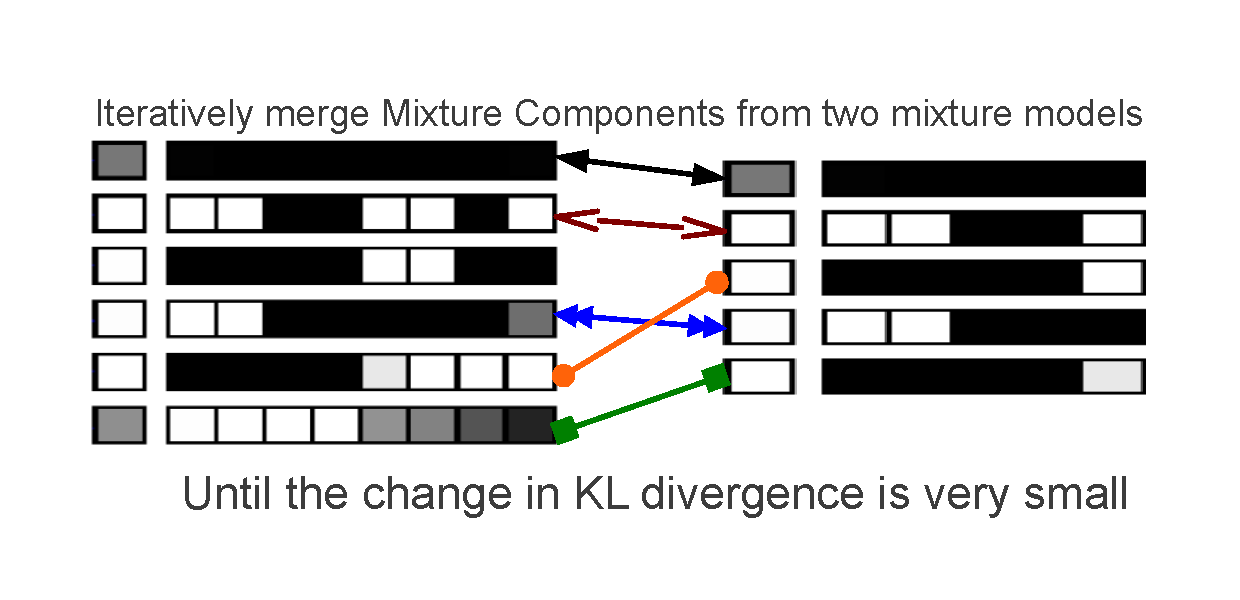
\includegraphics[trim=1.2cm 0cm 0cm 1cm, clip=true,width=0.72\textwidth]{figures/idasecondpage}
\end{figure}
\vspace{-7mm}
\scriptsize\item How is it done?
\scriptsize \item Fast approximation of KL divergence (P. R. Adhikari, J. Hollm\'en, DS 2012) \\ %\textcolor {red} {($\approx 10000$ times faster)}
\scriptsize
\textcolor{blue} {$KL  =  \displaystyle \sum_{i \in X^{*}} \pi_{\alpha} \displaystyle
\prod _{m=1}^{{d}}
\left(\alpha_m^{X^{*}_{im}}(1-\alpha_{m})^{(1-X^{*}_{im})} \right) -
\displaystyle \sum_{i{\prime} \in Y^{*}} \pi_{\beta} \displaystyle \prod
_{n=1}^{{d^{\prime}}} \left(
\beta_{n}^{Y^{*}_{i{\prime}n}}(1-\beta_{n})^{(1-Y^{*}_{i{\prime}n})} \right)
$}
\scriptsize \item Retrain the mixture models in different resolutions
\end{itemize}
\FrameText{P. R. Adhikari, J. Hollm{\'e}n, ACML'2012 \\ \vspace{-2mm} \textbf{Multiresolution Mixture Modeling using Merging of Mixture Components}}
\end{frame}
%%%%%%%%%%%%%%%%%%%%%%%%%%%%%%%%%%%%%%%%%%%%%%%%%%%%%%%%%%%%%%%%%%%%%%%%%%%%%%%%%%%%%%%%%%%%%

\begin{frame}{Performance of Multiresolution Mixture Model}
\vspace{-8mm}
\begin{figure}
\centering
  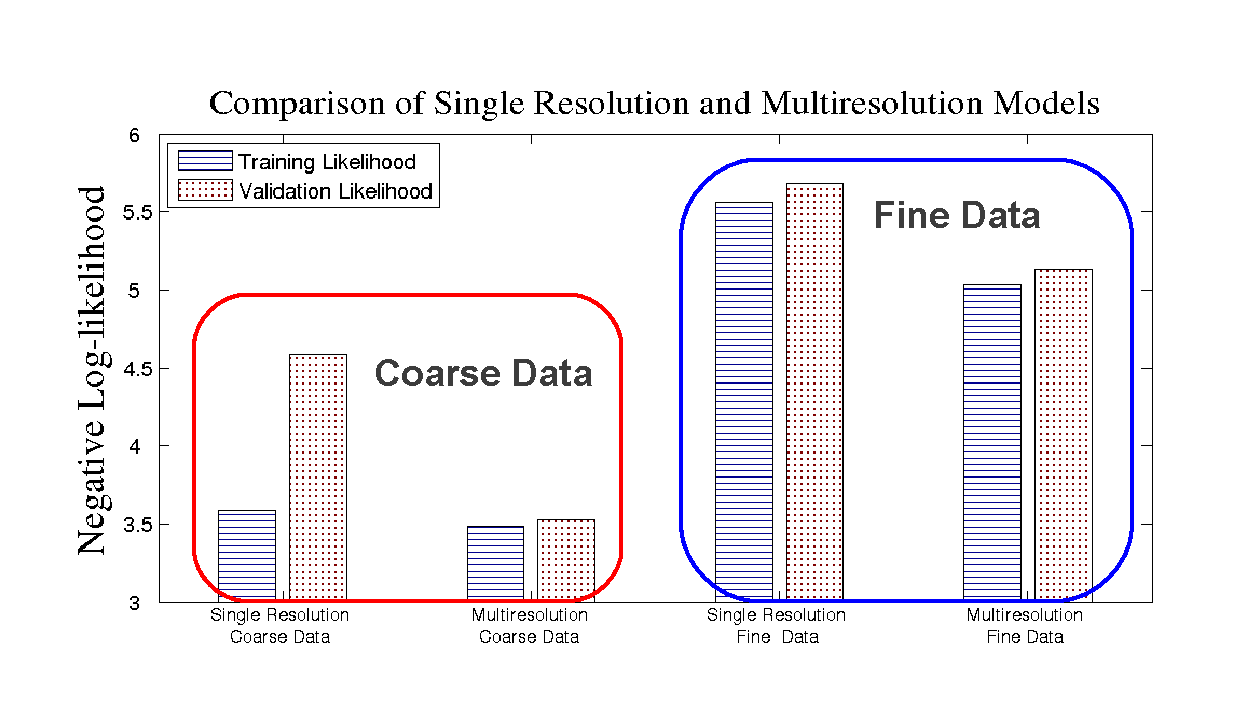
\includegraphics[trim=1.2cm 0cm 0cm 1cm, clip=true, width=0.97\textwidth]{figures/nbarlkhood}  
\end{figure}

\vspace{-10mm}

\scriptsize \hspace{15mm} Better generalization through merging of mixture components

\FrameText{P. R. Adhikari, J. Hollm{\'e}n, ACML'2012 \\ \vspace{-1mm} \textbf{Multiresolution Mixture Modeling using Merging of Mixture Components}}
\end{frame}

%%%%%%%%%%%%%%%%%%%%%%%%%%%%%%%%%%%%%%%%%%%%%%%%%%%%%%%%%%%%%%%%%%%%%%%%%%%%%%%%%%%%%%%%%%%%%%%%%%%%%%%%%%%%%%%%%%%%%%%%%%%%%

\begin{frame} {Multiresolution Mixture Components} 

      \begin{figure}
      \centering
      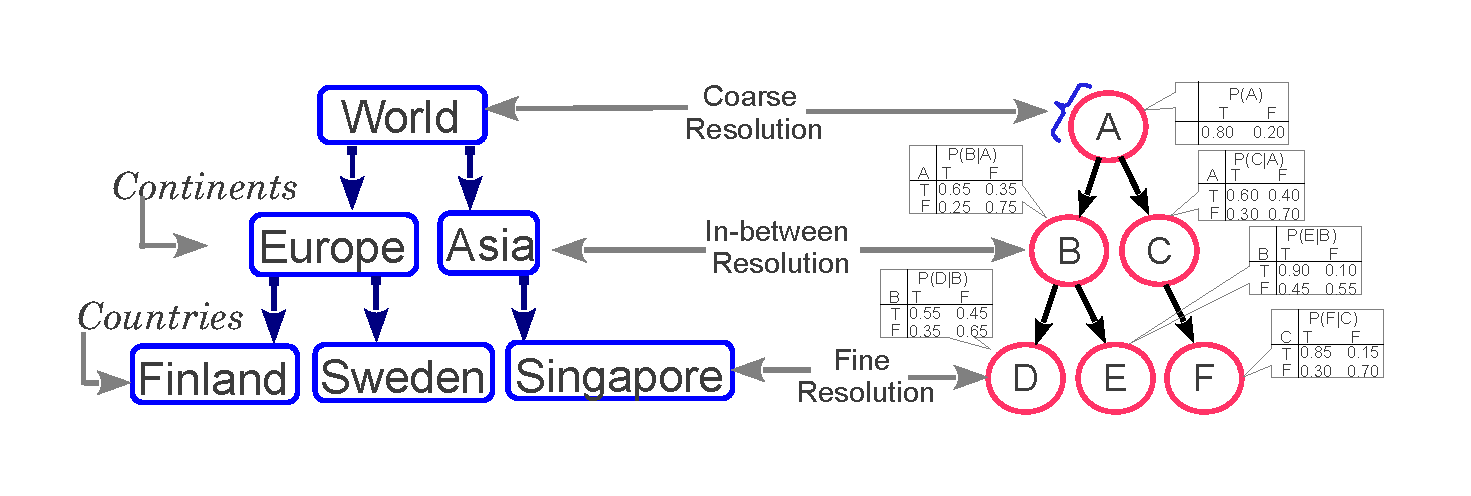
\includegraphics[trim=1cm 1cm 1cm 0cm, clip=true, width=0.9\textwidth]{figures/bnnfig1}
      \end{figure}
      
      \begin{itemize}\setlength{\itemsep}{2.5mm}
\item Domain ontology provides information about relationships between features in different resolutions
\item We can create a tree structure where features in the coarse resolution form the root and features in the fine resolution leaves of the tree
\end{itemize}
\FrameText{P. R. Adhikari, J. Hollm{\'e}n, DS'2013 \\ \vspace{-2mm} \textbf{Mixture Models from Multiresolution 0-1 Data.}}
\end{frame}
%\item We can represent the tree as a Bayesian network on the assumption that the directed arrows originate from the features in the coarse resolution
%%%%%%%%%%%%%%%%%%%%%%%%%%%%%%%%%%%%%%%%%%%%%%%%%%%%%%%%%%%%%%%%%%%%%%%%%%%%%%%%%%%%%%%%%%%%%%%%%%%%%%%%%%%%%%%%%%


% \begin{frame} {Bayesian Networks to Impute Missing Resolutions} 
% 
%       \begin{figure}
%       \centering
%       \includegraphics[trim=1cm 1cm 1cm 1cm, clip=true, width=0.9\textwidth]{figures/frobiusn}
%       \end{figure}
%       
%       \begin{itemize}\setlength{\itemsep}{1mm}
%       
%       \small
% \item Bayesian networks can be used to impute missing resolutions using marginal inference. 
% \item For a joint distribution P(A,B,C) and an evidence B=true, marginal inference calculation is:
% \hspace{5mm} $P(A\mid B=true) \propto \displaystyle\sum_C P(A,B=true,C). $
% 
% 
% \end{itemize}
% \FrameText{P. R. Adhikari, J. Hollm{\'e}n, DS'2013 \\ \vspace{-2mm} \textbf{Mixture Models from Multiresolution 0-1 Data.}}
% 
% \end{frame}

%%%%%%%%%%%%%%%%%%%%%%%%%%%%%%%%%%%%%%%%%%%%%%%%%%%%%%%%%%%%%%%%%%%%%%%%%%%%%%%%%%%%%%%%%%%%%%%%%%%%%%%%%%%%%%%%%%


\begin{frame} {Structure of Mixture Model} 

      \begin{figure}
      \centering
      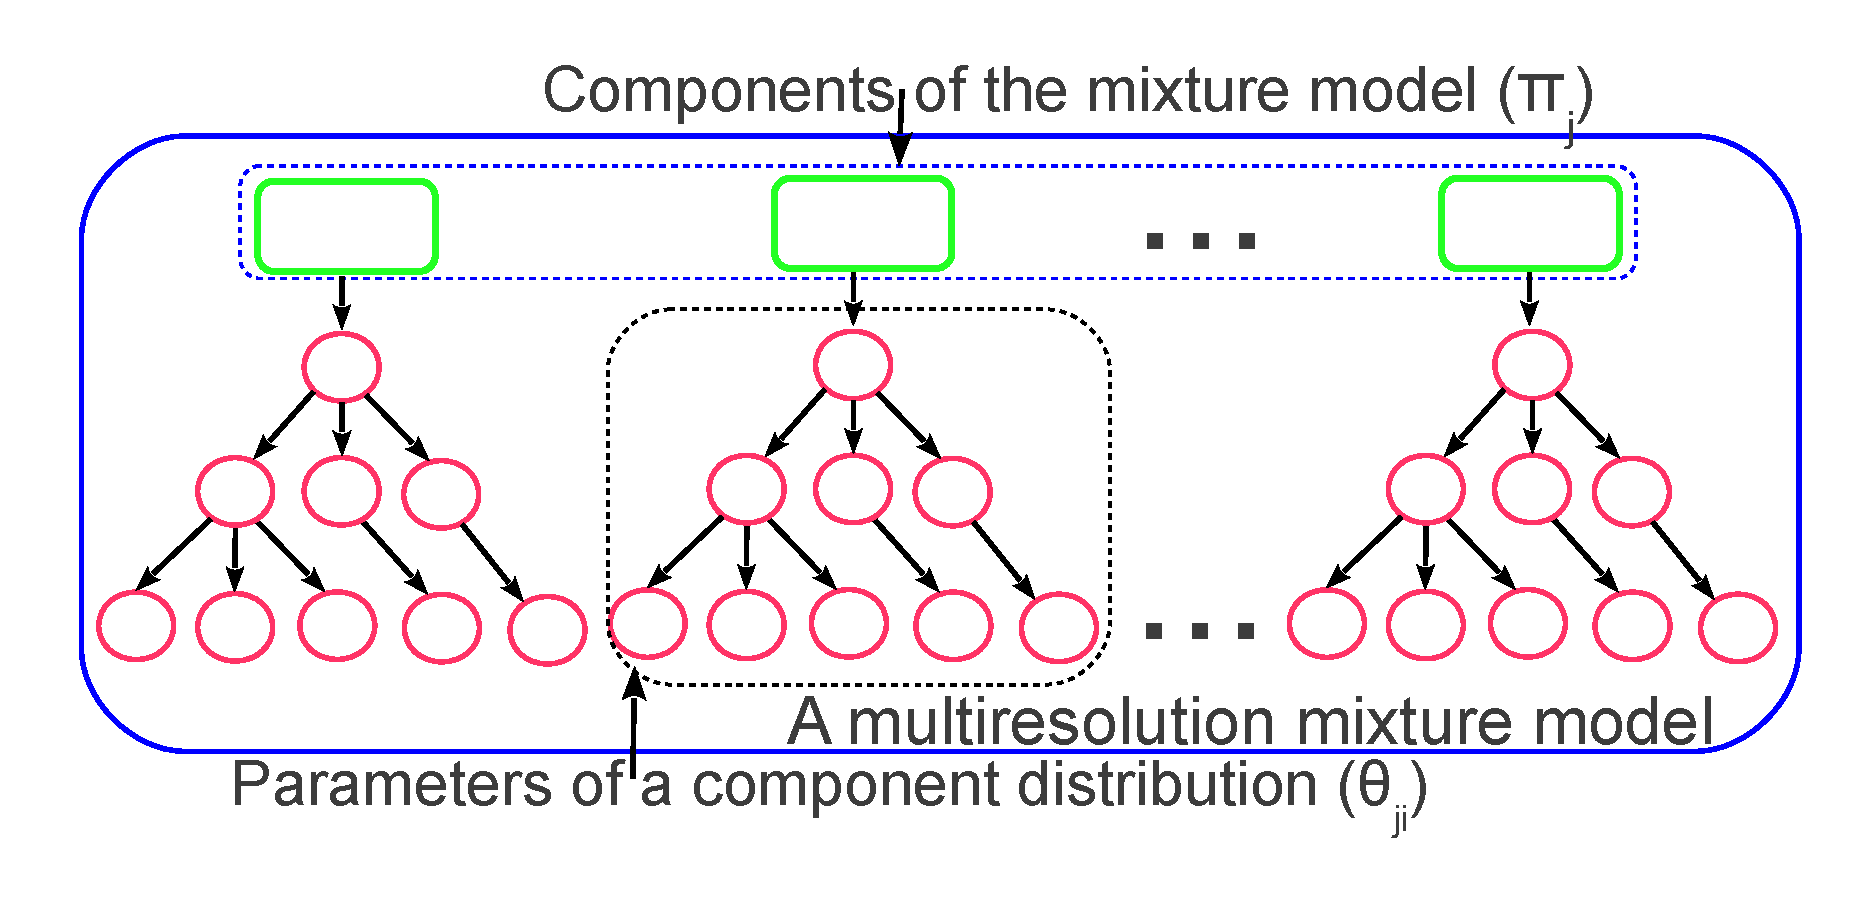
\includegraphics[trim=1cm 1.5cm 1cm 1cm, clip=true, width=0.9\textwidth]{figures/mixtrees}
      \end{figure}
      
      \begin{itemize}\setlength{\itemsep}{1mm}
      
\small
\item The components of the mixture model are Bayesian networks themselves 
\item Now, the problem is to learn the parameters $ \boldsymbol{\Theta}=\{J$, $\{ \pi_j,\theta_j\}_{j=1}^{J}\}$
\end{itemize}
\FrameText{P. R. Adhikari, J. Hollm{\'e}n, DS'2013 \\ \vspace{-2mm} \textbf{Mixture Models from Multiresolution 0-1 Data.}}

\end{frame}

%%%%%%%%%%%%%%%%%%%%%%%%%%%%%%%%%%%%%%%%%%%%%%%%%%%%%%%%%%%%%%%%%%%%%%%%%%%%%%%%%%%%%%%%%%%%%%%%%%%%%%%%%%%%%%%%%%

\begin{frame} {Multiresolution Mixture Model Results} 

      \begin{figure}
      \centering
      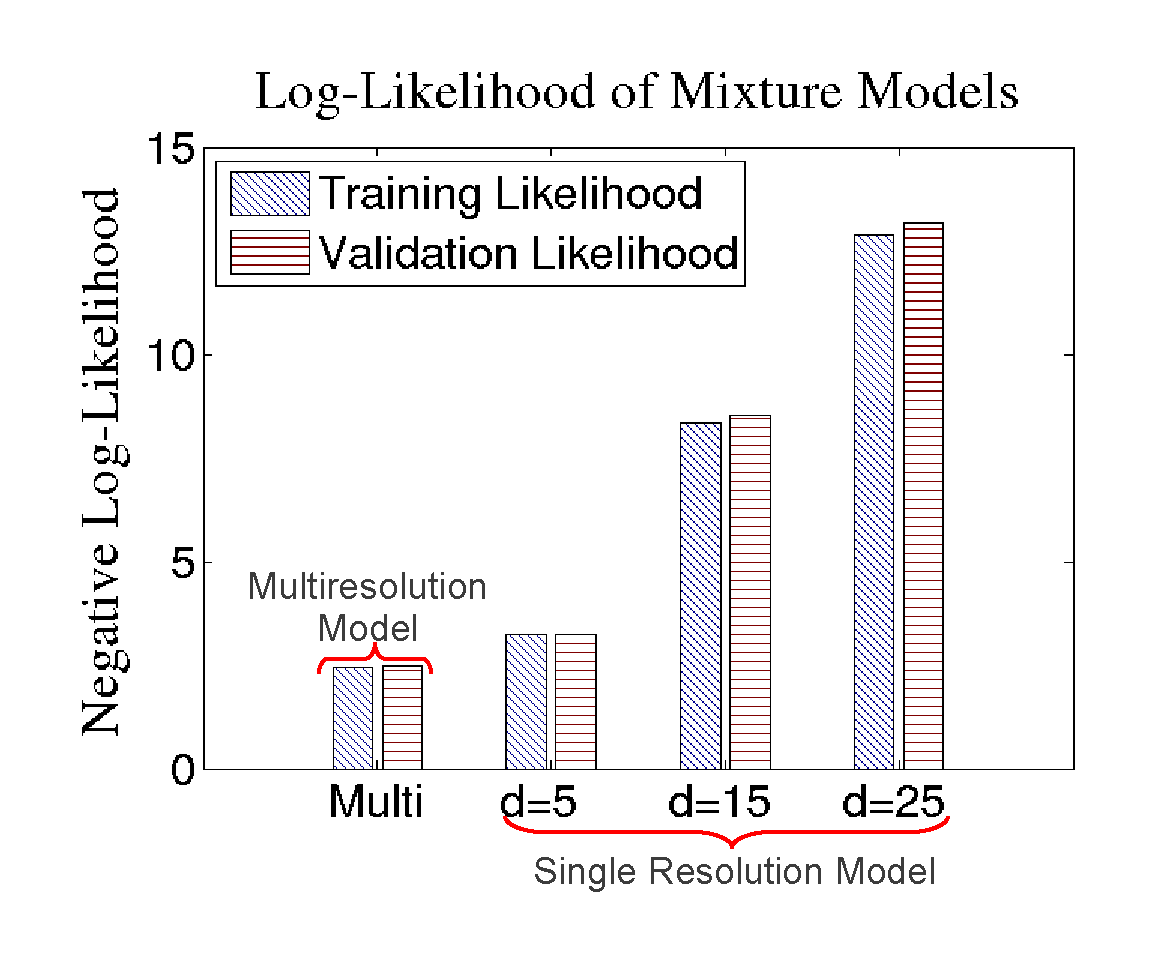
\includegraphics[trim=1cm 0.5cm 1cm 1cm, clip=true, width=0.5\textwidth]{figures/barlkhood}
      \end{figure}
      
      \vspace{-5mm}
      
      \begin{itemize}\setlength{\itemsep}{1mm}
      
\small
\item The Y-axis shows the negative log likelihood, therefore, the shorter the bar, better the result
\item The multiresolution model outperforms single resolution models
\end{itemize}
\FrameText{P. R. Adhikari, J. Hollm{\'e}n, DS'2013 \\ \vspace{-2mm} \textbf{Mixture Models from Multiresolution 0-1 Data.}}

\end{frame}

%%%%%%%%%%%%%%%%%%%%%%%%%%%%%%%%%%%%%%%%%%%%%%%%%%%%%%%%%%%%%%%%%%%%%%%%%%%%%%%%%%%%%%%%%%%%%%%%%%%%%%%%%%%%%%%%%%

\begin{frame}{Summary and Conclusions}

\begin{itemize} \setlength{\itemsep}{5.5mm}
 \item Mixture Modeling of Multiresolution 0--1 Data in three ways:
 \begin{itemize} \setlength{\itemsep}{4mm}
  \item Data Transformation 
  \item Merging of mixture components
  \item Bayesian network as component distributions
 \end{itemize}
 \item Experiments on multiresolution chromosomal datasets
 \item Experiments show that multiresolution models outperform single resolution models
\end{itemize}
\end{frame}


%%%% QUESTIONS FRAME BELOW %%%%%%
%%%%%%%%%%%%%%%%%%%%%%%%%%%%%%%%%%%%%%%%%%%%%%%%%%%%%%%%%%%%%%%%%%%%%%%%%%%%%%%%%%%%%%%%%%%%%



\begin{frame}
 \frametitle{Questions, Comments, Feedback and Acknowledgment}
 \begin{figure}[h!]
 \centering
 
\includegraphics[width=0.5\textwidth]{figures/questions}
 \end{figure}
 
 \vspace{-15mm}
 
 \begin{figure}[h!]
 \centering
 
\includegraphics[width=0.8\textwidth]{figures/logoslong}
 \end{figure}
 
 \vspace{-5mm}
 
 \small The work is funded by Helsinki Doctoral Programme in Computer Science--Advanced Computing and Intelligent Systems (Hecse)
 \end{frame}
 
%%%%%%%%%%%%%%%%%%%%%%%%%%%%%%%%%%%%%%%%%%%%%%%%%%%%%%%%%%%%%%%%%%%%%%%%%%%%%%%%%%%%%%%%%%%%%
\end{document}
